\subsection{Encoding via ResNet50}

\begin{figure}[!ht]
    \centering
    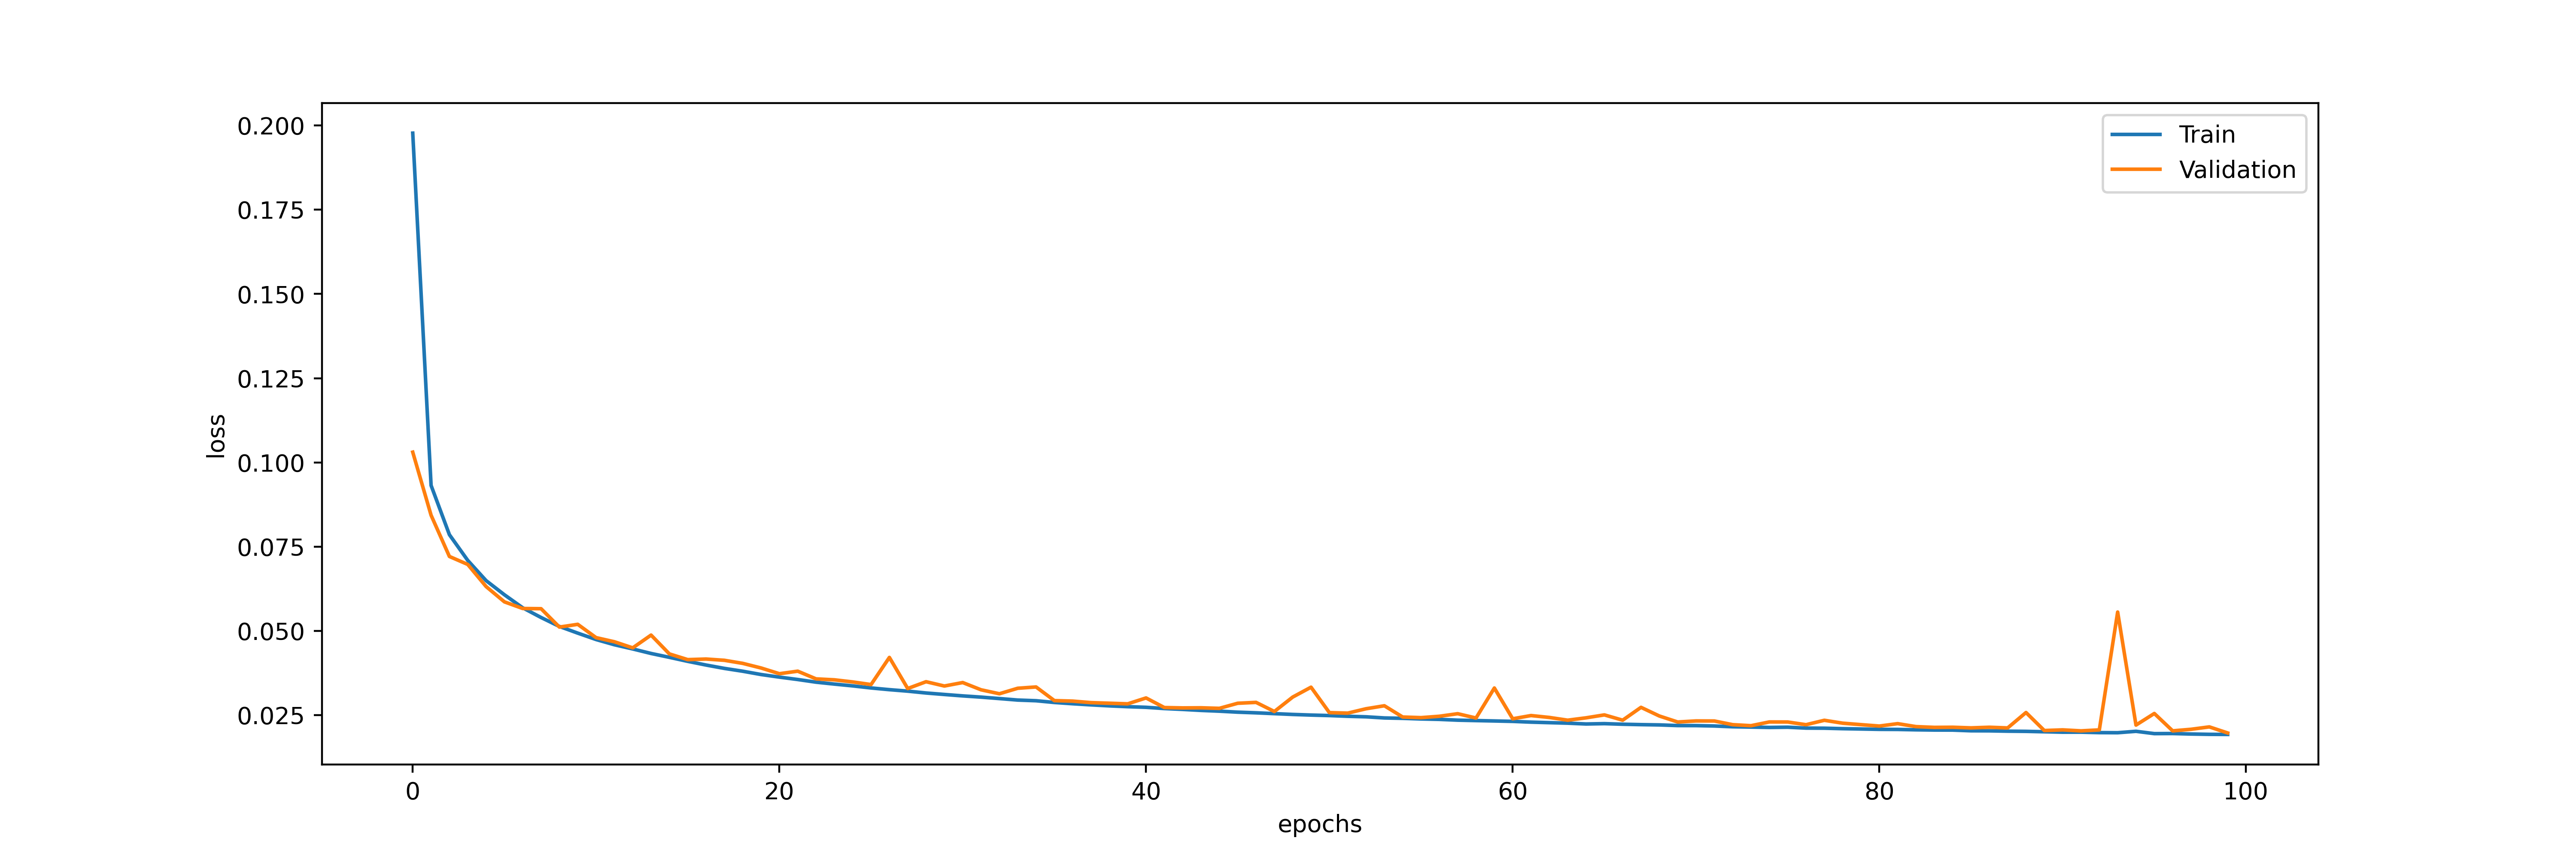
\includegraphics[width=\textwidth,trim={0 1cm 0 1cm},clip]{./results/resnet50_vgg19/20230514_213740_results.png}
    \caption{Learning curve of the ResNet50 Encoder}
    \label{fig:resnet50_learning_curve}
\end{figure}



\begin{figure}[!ht]
    \centering
    \begin{subfigure}{\textwidth}
        \centering
        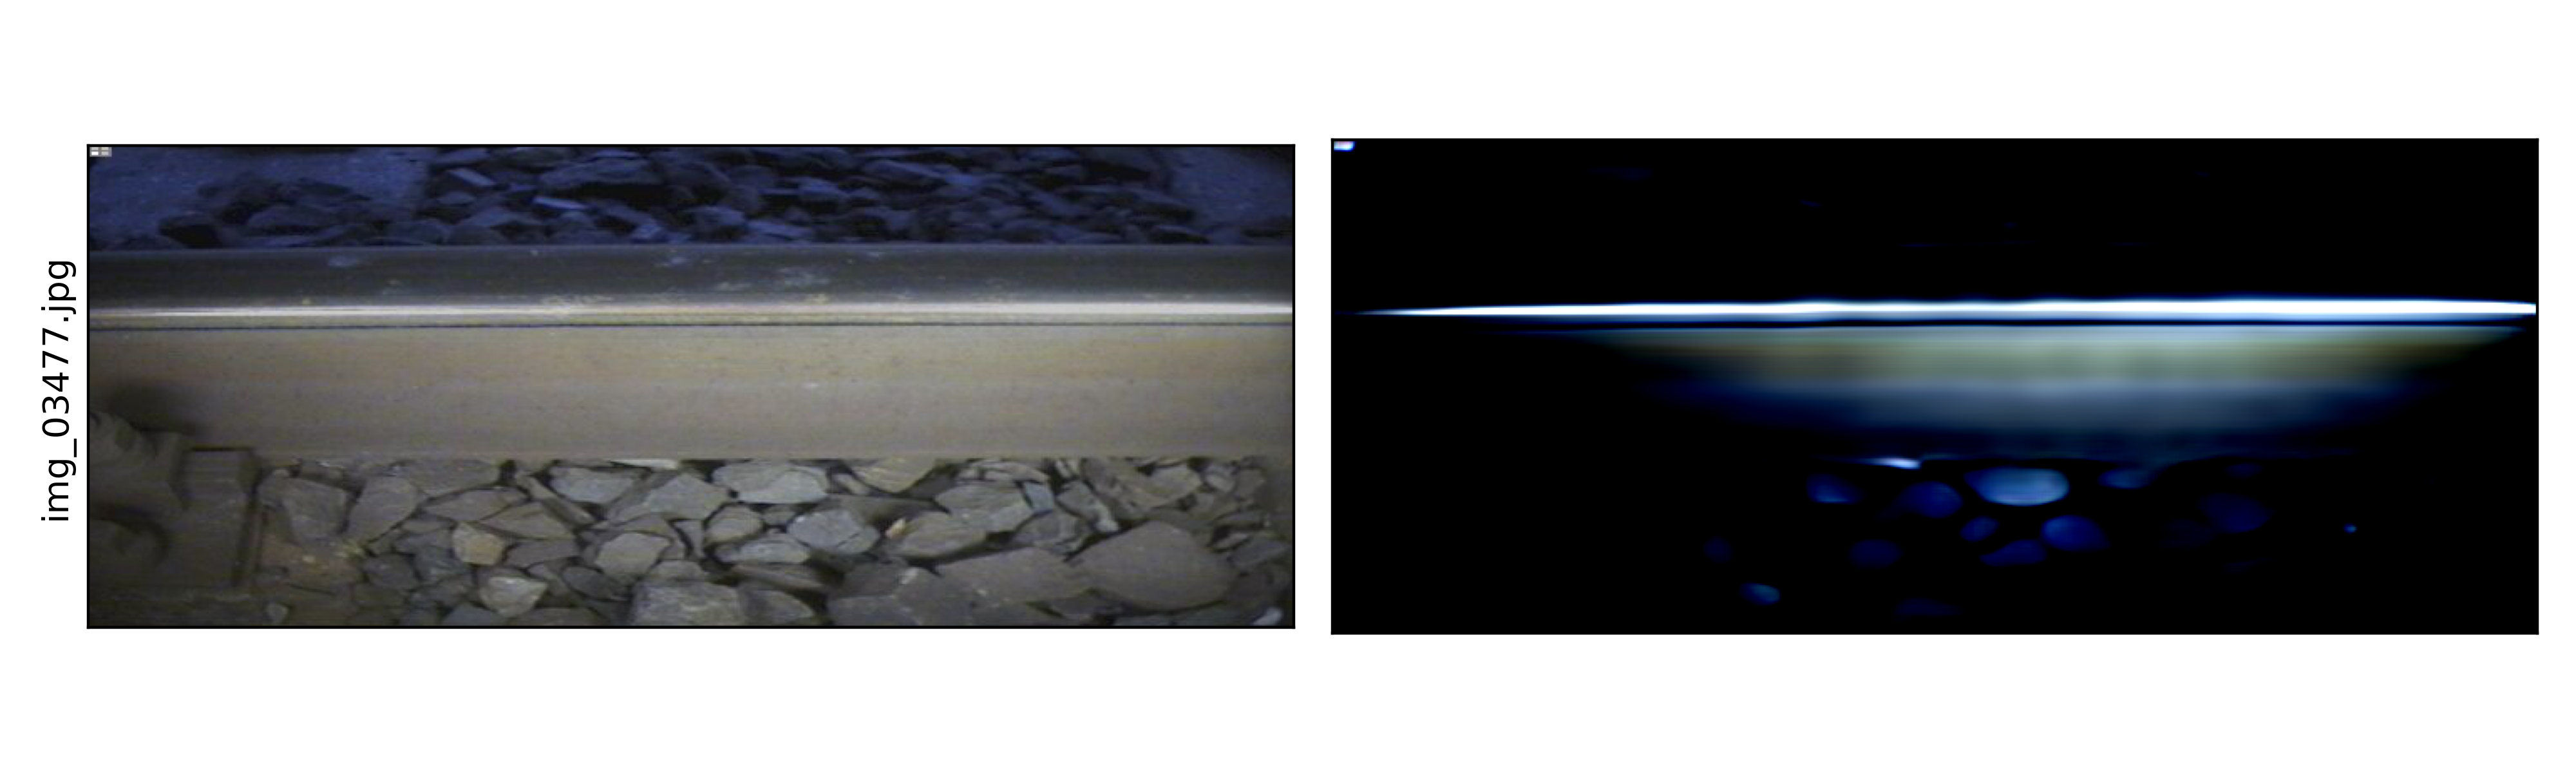
\includegraphics[width=0.9\textwidth,trim={0 1cm 0 1cm},clip]{./results/resnet50_vgg19/20230514_213740_predict_0.png}
    \end{subfigure}
    \begin{subfigure}{\textwidth}
        \centering
        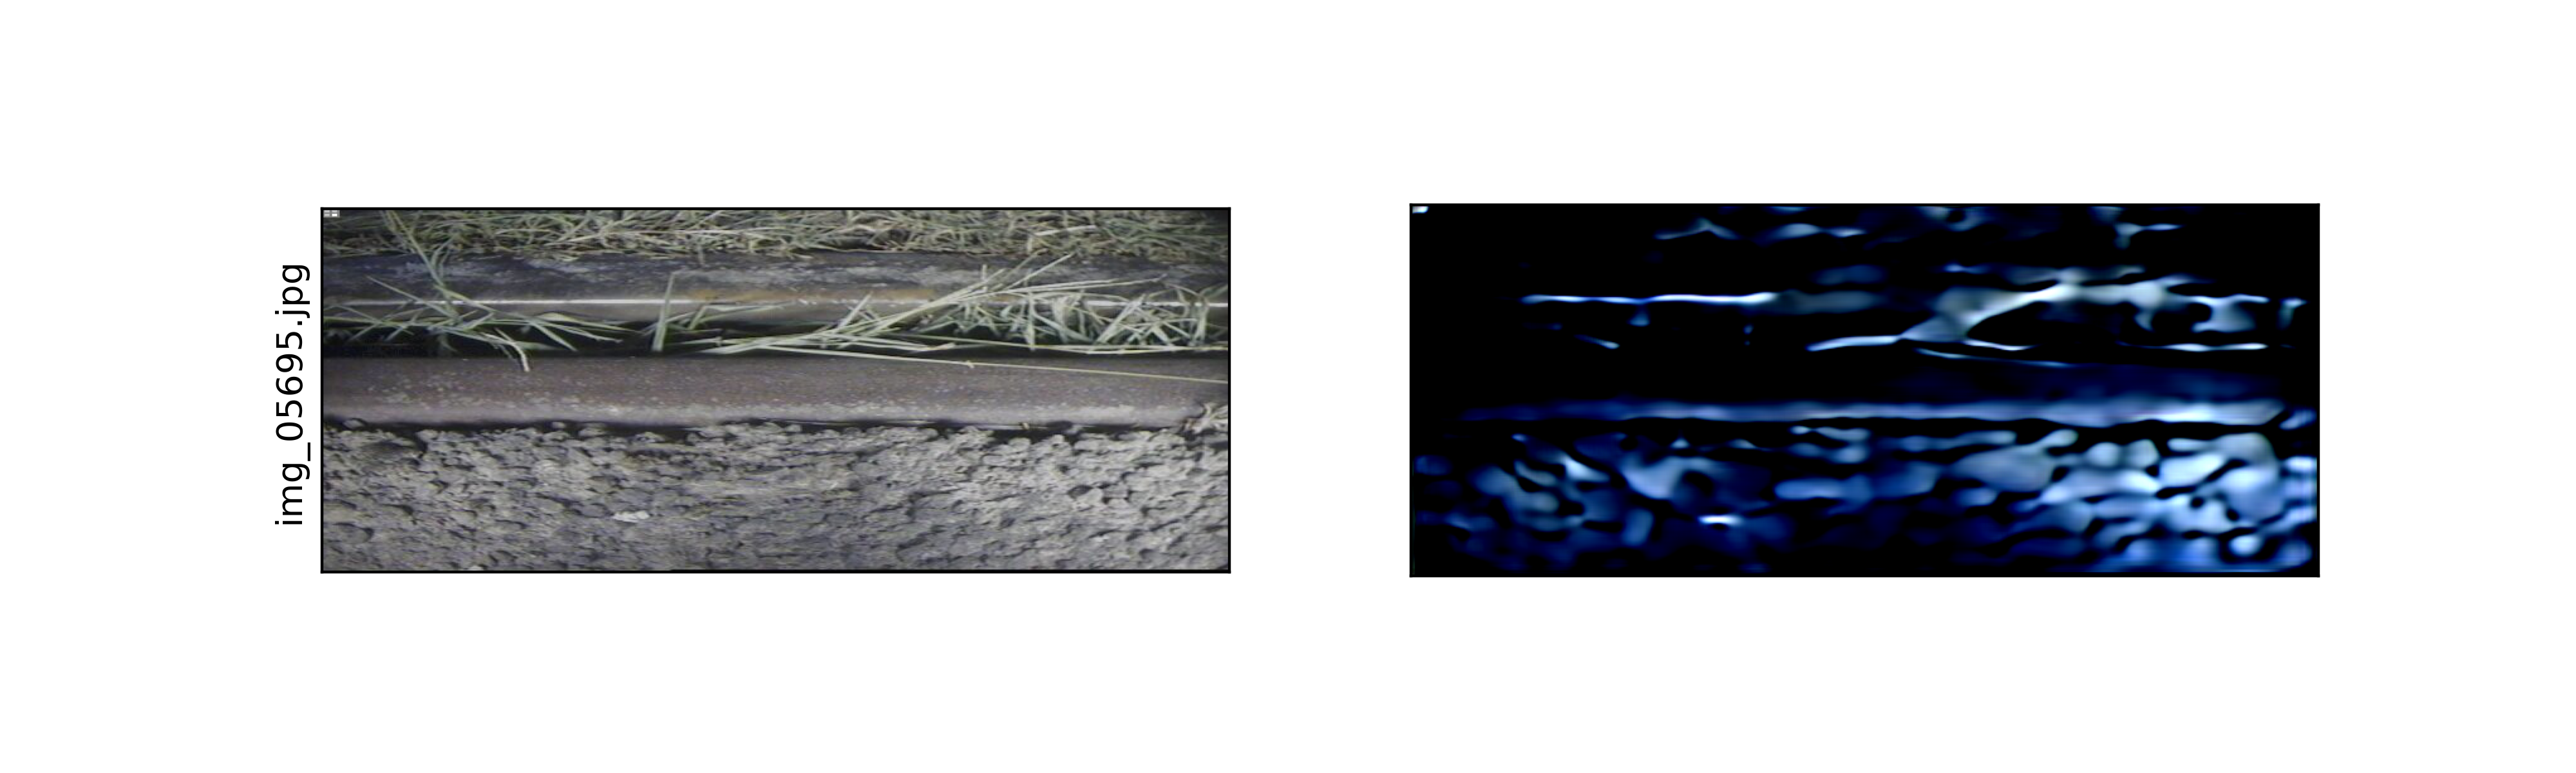
\includegraphics[width=0.9\textwidth,trim={0 1cm 0 1cm},clip]{./results/resnet50_vgg19/20230514_213740_predict_1.png}
    \end{subfigure}
    \begin{subfigure}{\textwidth}
        \centering
        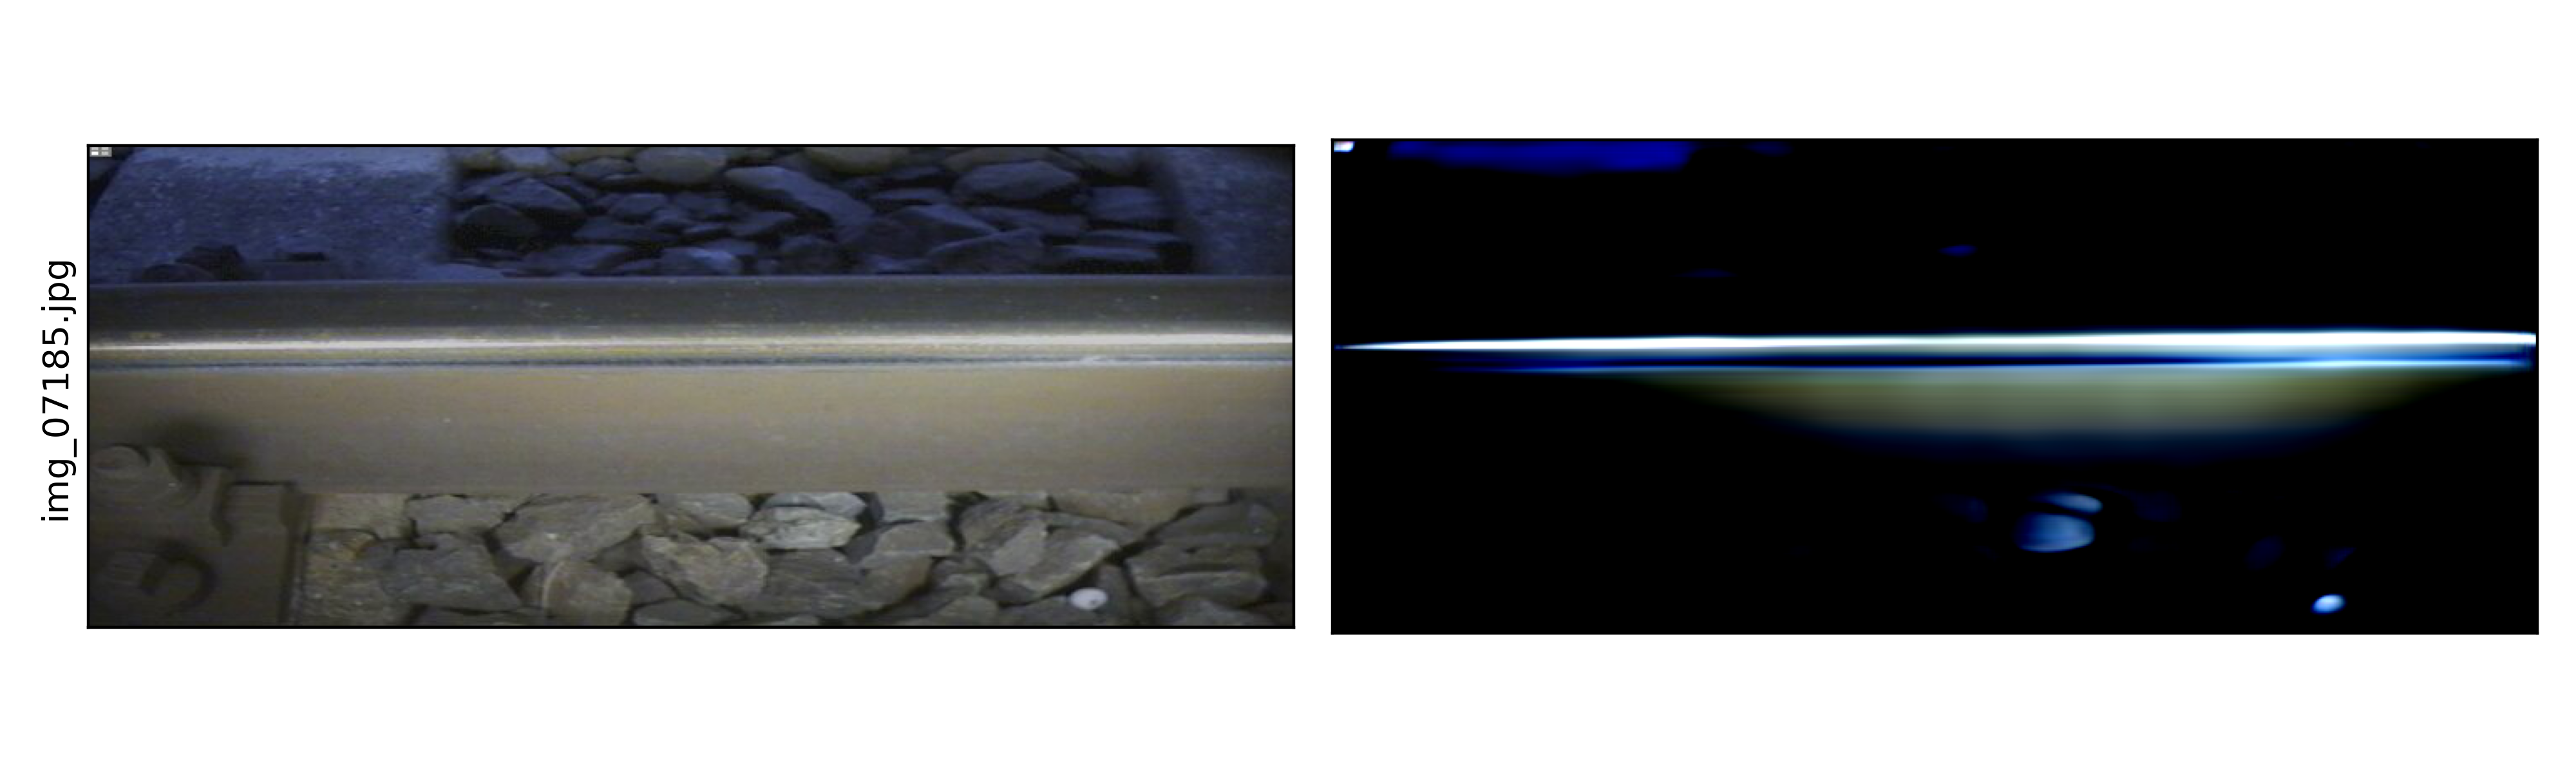
\includegraphics[width=0.9\textwidth,trim={0 1cm 0 1cm},clip]{./results/resnet50_vgg19/20230514_213740_predict_2.png}
    \end{subfigure}
    \caption{Predicted images in case of ResNet50 Encoder}
    \label{fig:resnet50_examples}
\end{figure}



\begin{figure}[!ht]
    \centering
    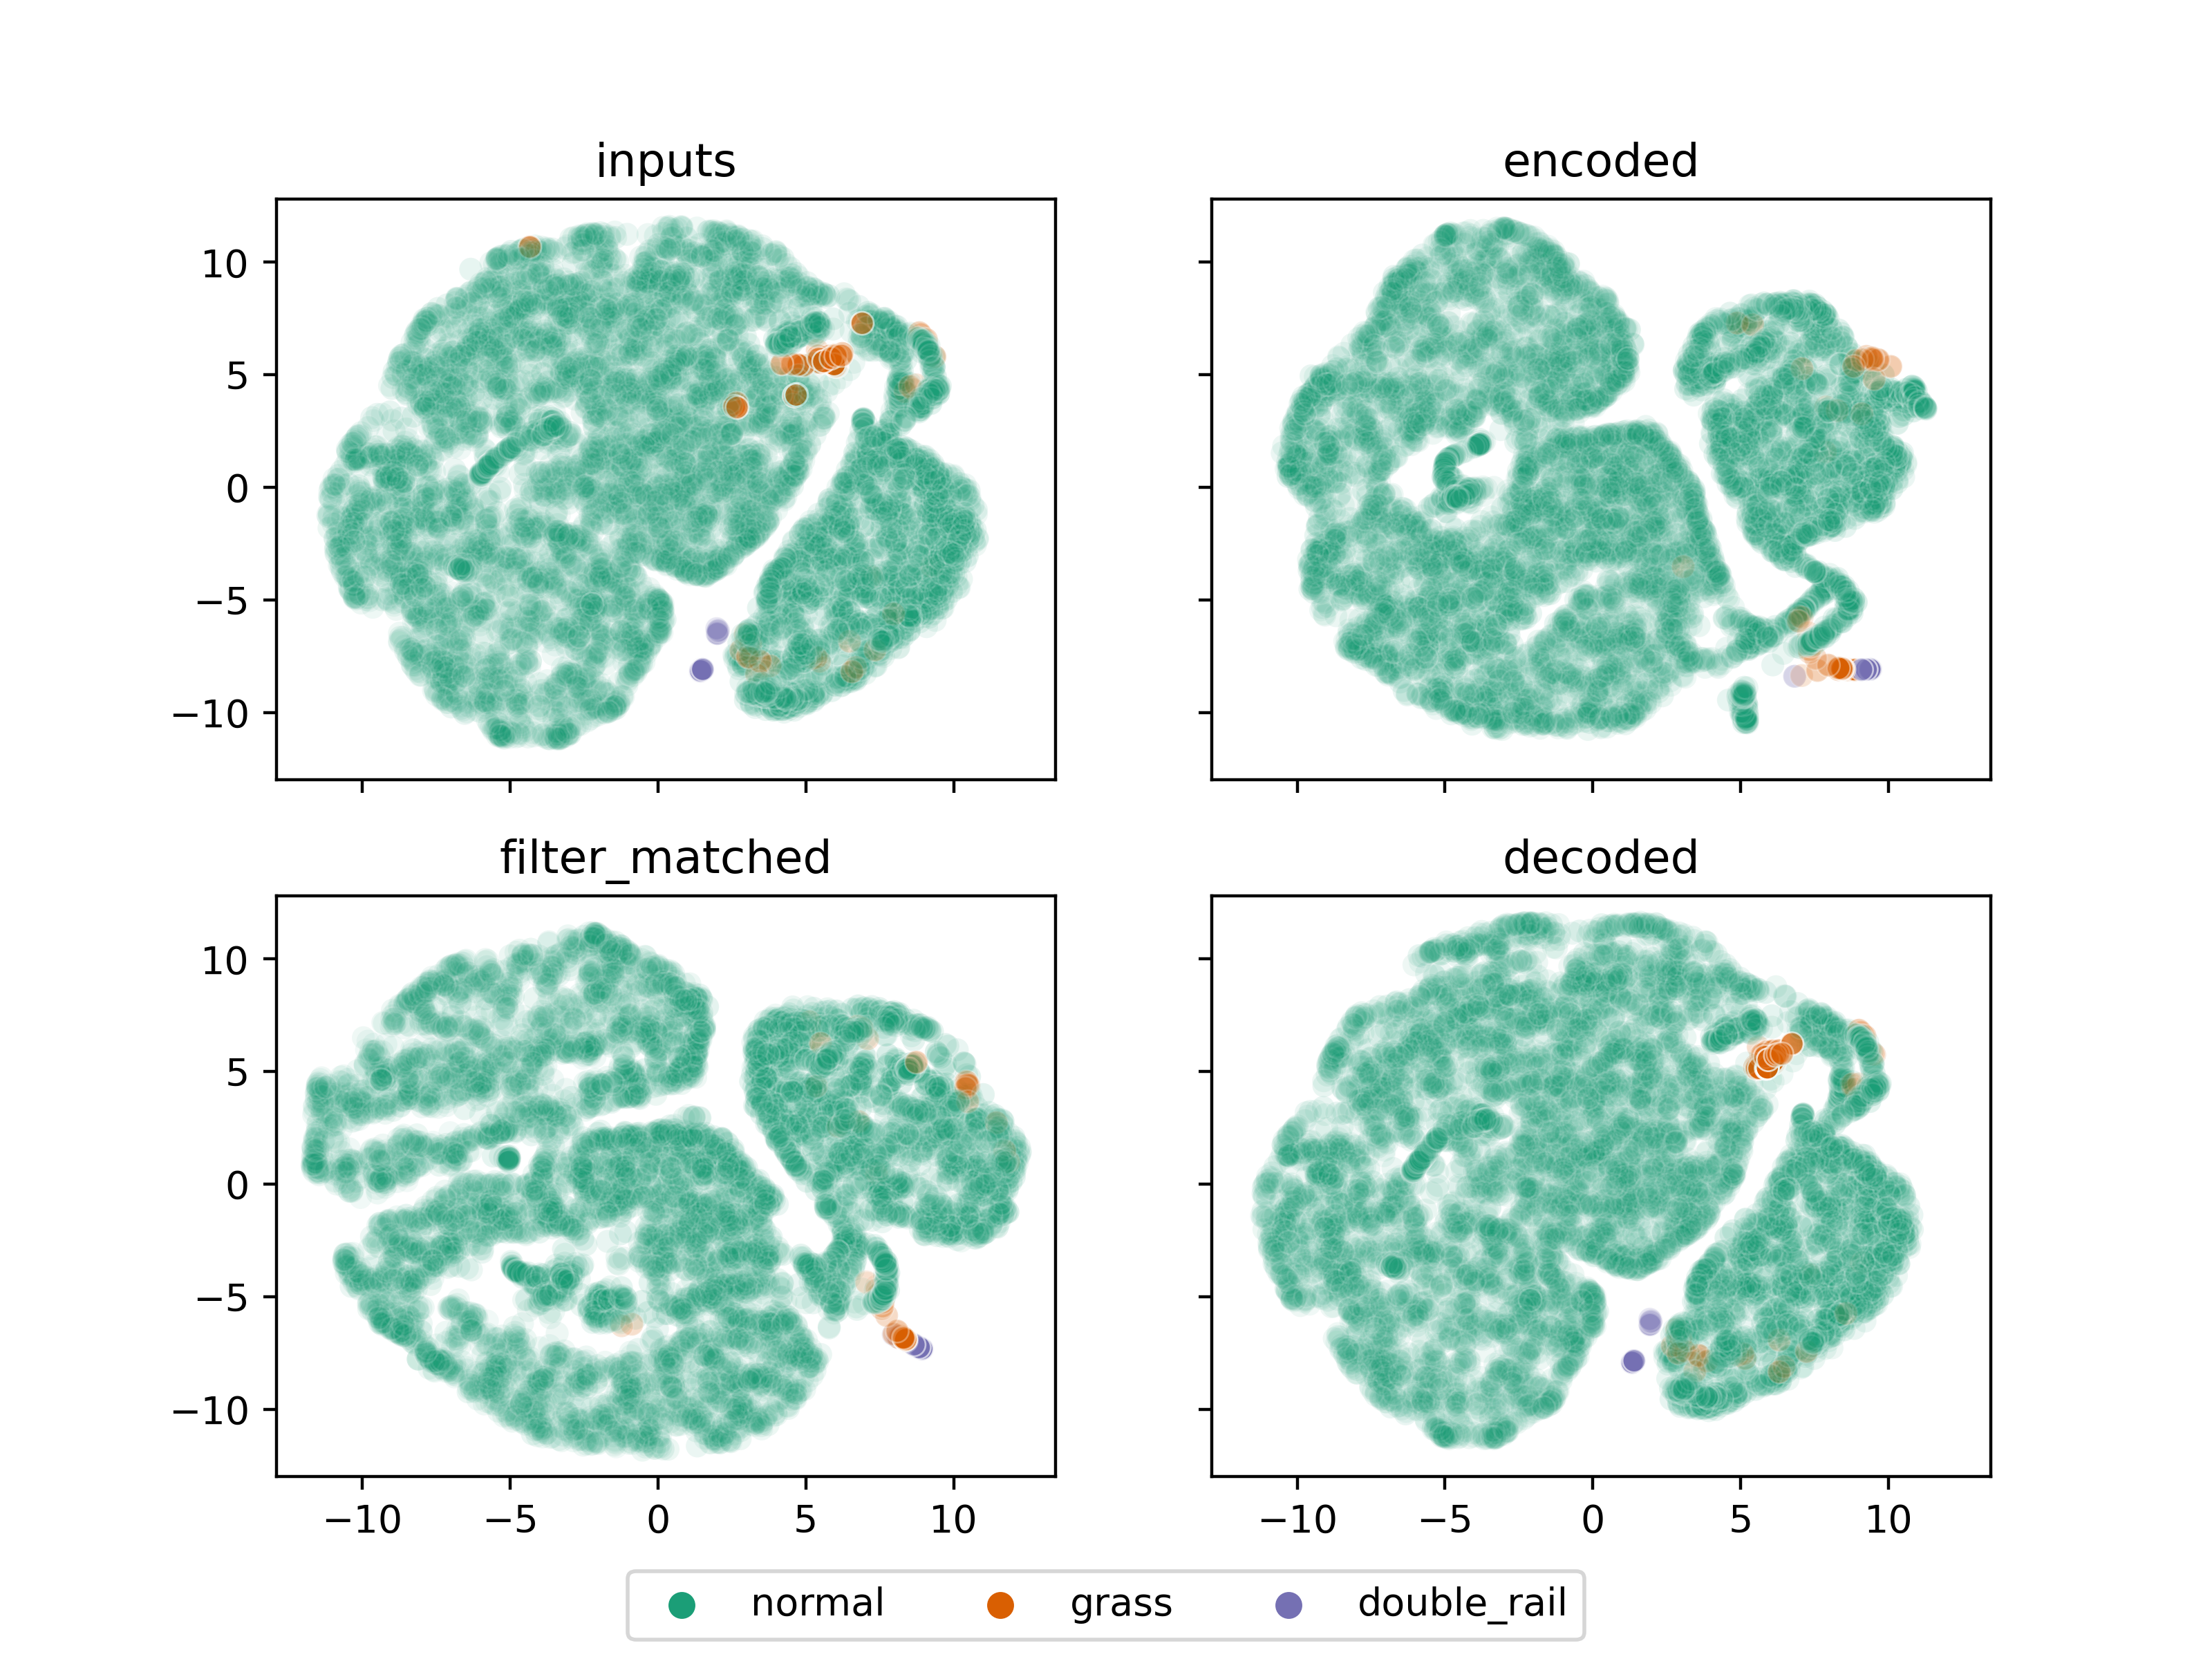
\includegraphics[width=\textwidth,trim={0 1cm 0 1cm},clip]{./results/resnet50_vgg19/20230514_213740_feature_vectors_1.png}
    \caption{PCA / t-SNE visualization of the ResNet50 Encoder}
    \label{fig:resnet50_pca}
\end{figure}



\begin{figure}[!ht]
    \centering
    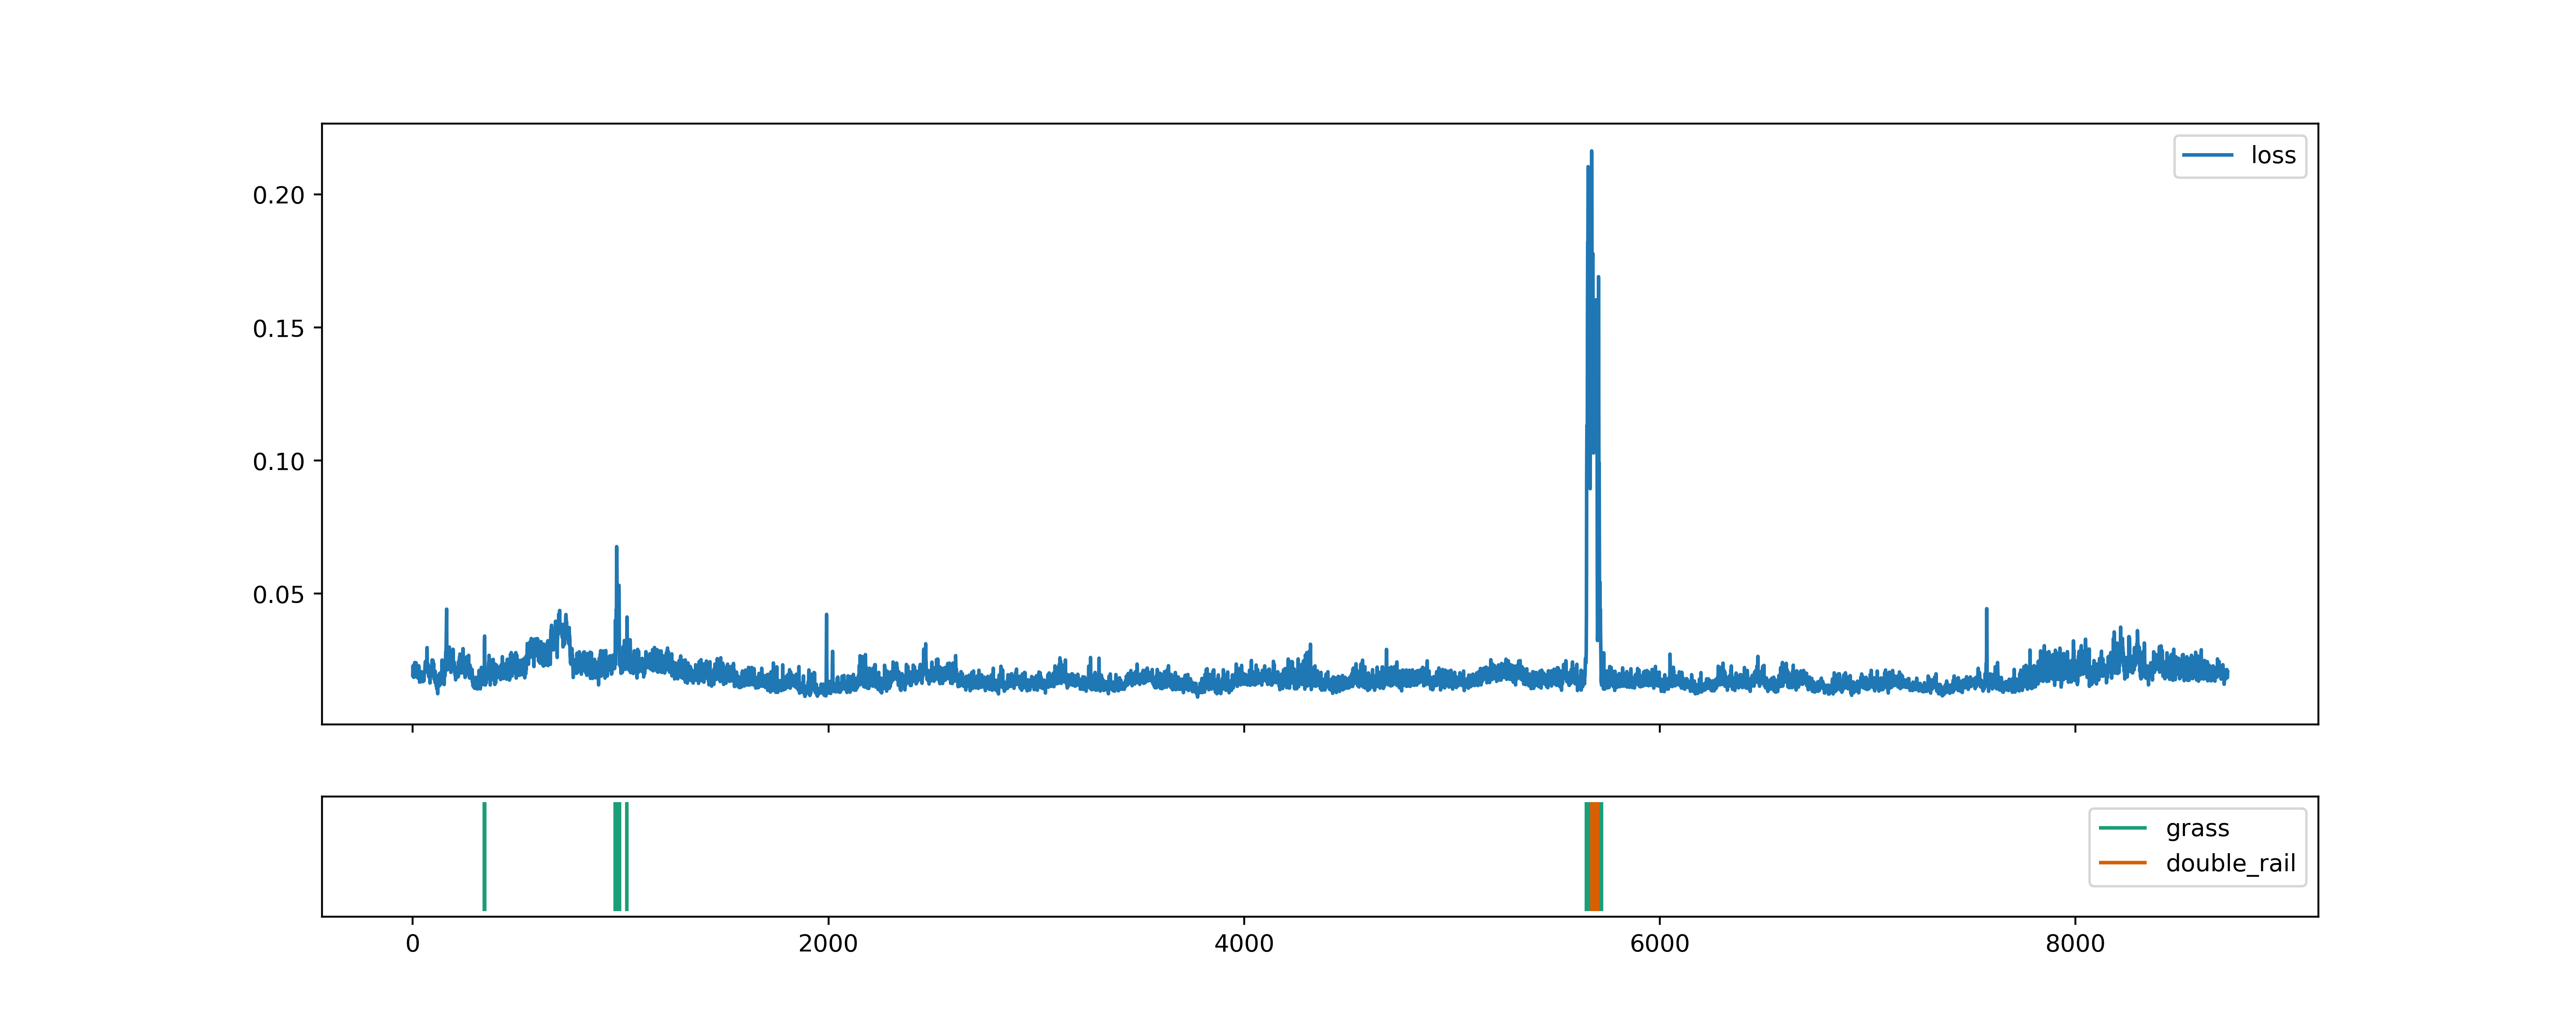
\includegraphics[width=\textwidth,trim={0 1cm 0 1cm},clip]{./results/resnet50_vgg19/20230514_213740_feature_vectors_loss.png}
    \caption{Loss values of the dataset with ResNet50 encoding}
    \label{fig:resnet50_loss}
\end{figure}



\begin{figure}[!ht]
    \centering
    \begin{subfigure}{0.4\textwidth}
        \centering
        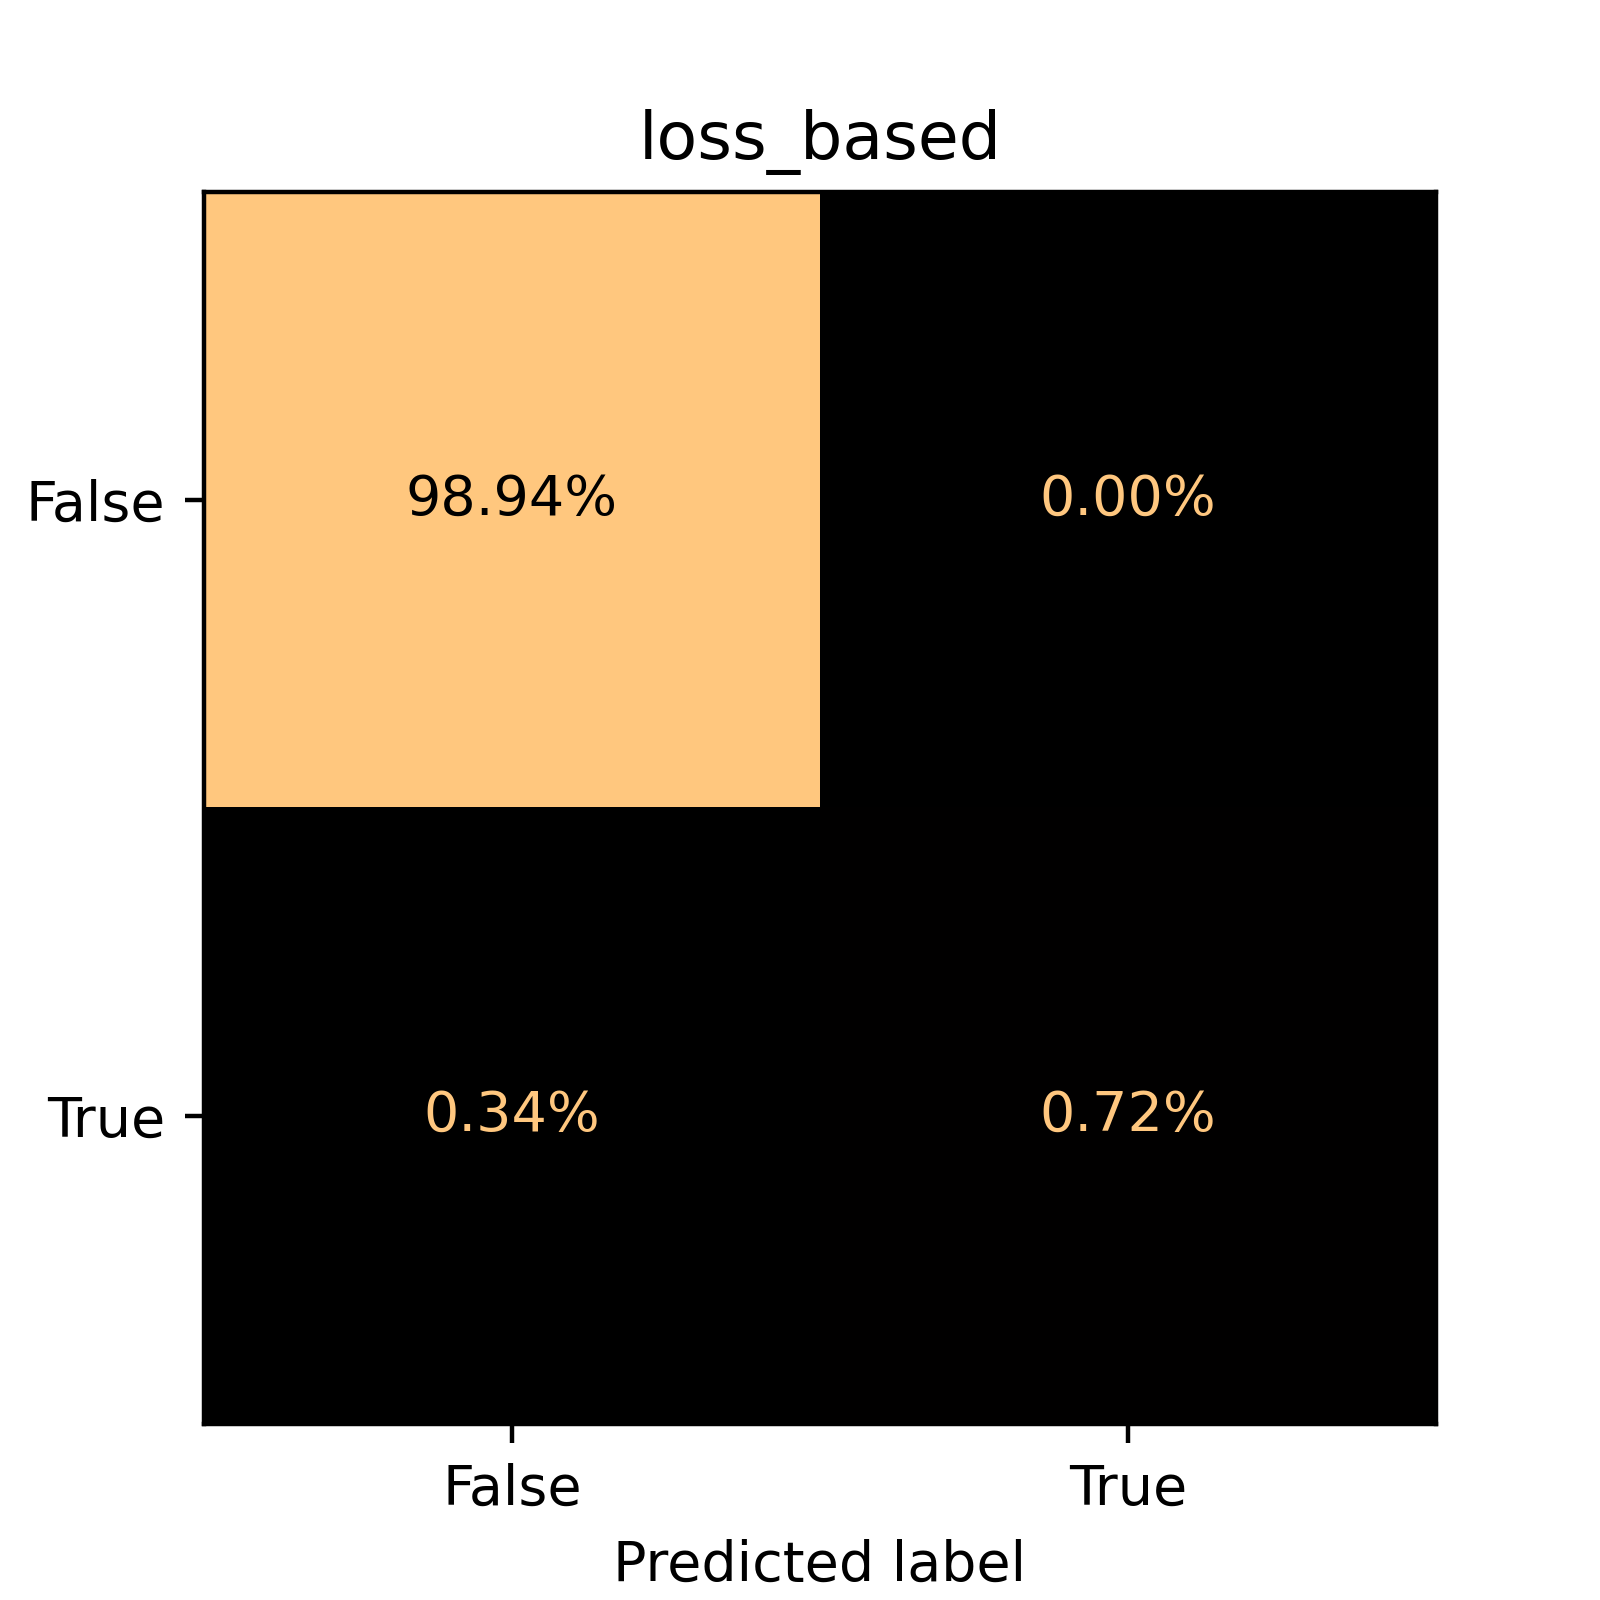
\includegraphics[width=\textwidth,trim={0 1cm 0 1cm},clip]{./results/resnet50_vgg19/20230514_213740_loss_based_cm.png}
    \end{subfigure}
    \begin{subfigure}{0.4\textwidth}
        \centering
        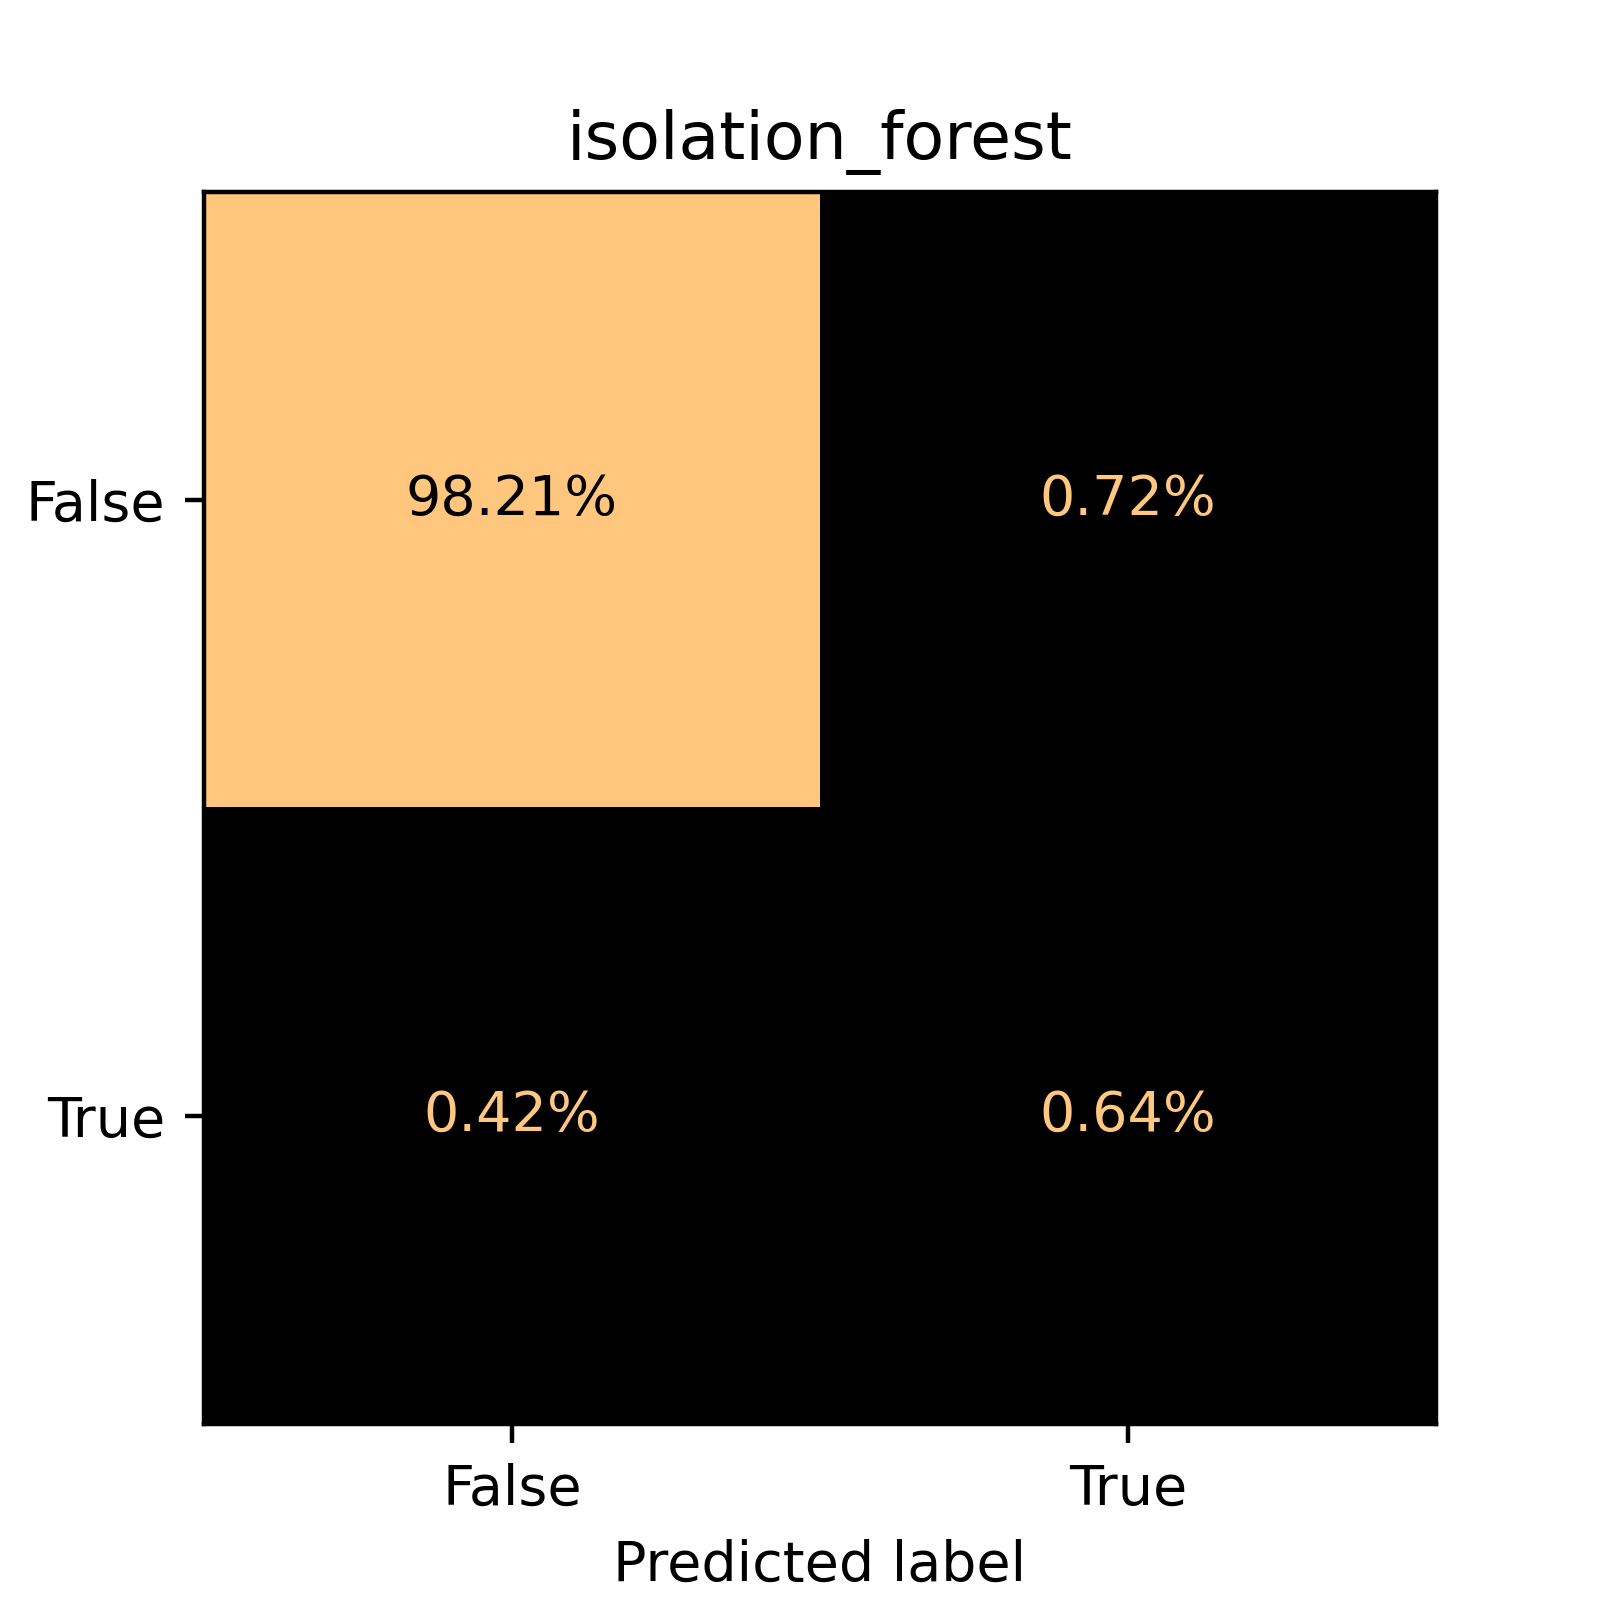
\includegraphics[width=\textwidth,trim={0 1cm 0 1cm},clip]{./results/resnet50_vgg19/20230514_213740_isolation_forest_cm.png}
    \end{subfigure}
    \caption{Confusion Matrices of the ResNet50 Encoder}
    \label{fig:resnet50_cm}
\end{figure}